%% ------------------------------------------------------------------------- %%
\chapter{Conceitos}
\label{cap:conceitos}

%% ------------------------------------------------------------------------- %%
\section{Registro}\index{Registro}
\label{sec:fundamentos}

  O registro tem como objetivo alinhar uma imagem, a imagem alvo (\textit{IA}),
geometricamente à outra imagem, a imagem referência (\textit{IR}). O alinhamento
é realizado por uma função de alinhamento, que parte de correspondência entre os
pontos de controle das duas imagens para definir seus parâmetros, encontrando uma
solução que mapeia todos os pontos da imagem referência para pontos da imagem alvo
dada uma deformação.

  Os algoritmos de registro podem ser divididos, com algumas ressalvas, em cinco
passos gerais:
\begin{enumerate}
    \item Pré-processamento;
    \item Detecção de características;
    \item Correspondência de características;
    \item Estimativa da função de transformação;
    \item Reamostragem da imagem Alvo.
\end{enumerate} % TODO: Colocar o diagrama aqui %

\begin{figure}[H]
    \centering
    \begin{subfigure}[t]{0.3\textwidth}
      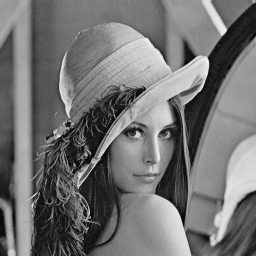
\includegraphics[width=\textwidth]{figuras/static.png}
      \subcaption*{(a)}
      \label{fig:ref-image}
    \end{subfigure}
    \begin{subfigure}[t]{0.3\textwidth}
      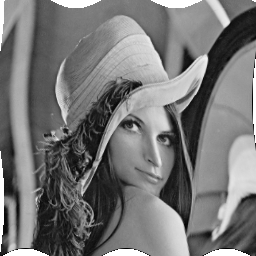
\includegraphics[width=\textwidth]{figuras/lenaMoving.png}
      \subcaption*{(b)}
      \label{fig:sin-image}
    \end{subfigure} \\
    \begin{subfigure}[t]{0.64\textwidth}
      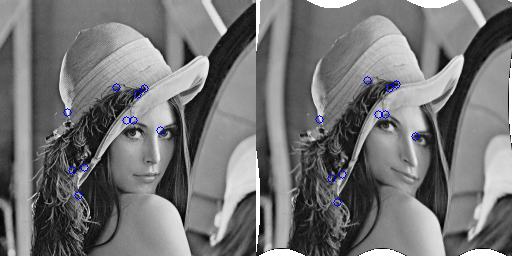
\includegraphics[width=\textwidth]{figuras/Features.png}
      \subcaption*{(c)}
      \label{fig:featuresSIFT}
    \end{subfigure} \\
    \begin{subfigure}[t]{0.64\textwidth}
      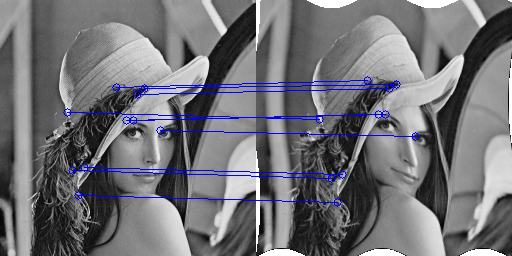
\includegraphics[width=\textwidth]{figuras/MatchedFeatures.png}
      \subcaption*{(d)}
      \label{fig:MatchedFeatures}
    \end{subfigure} \\
    \begin{subfigure}[t]{0.3\textwidth}
      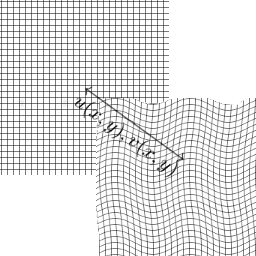
\includegraphics[width=\textwidth]{figuras/estimativa.png}
      \subcaption*{(e)}
      \label{fig:estimativa}
    \end{subfigure}
    \begin{subfigure}[t]{0.3\textwidth}
      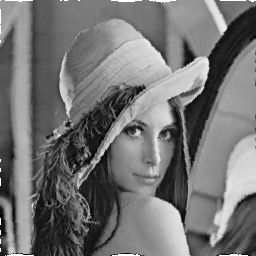
\includegraphics[width=\textwidth]{figuras/lenaRegistrada.png}
      \subcaption*{(f)}
      \label{fig:lenaRegistrada}
    \end{subfigure}
    \caption{Exemplo de uma instância de registro. (a) Imagem Referência.
             (b) Imagem Alvo deformada artificialmente.
             (c) Detecção de características utilizando o SURF.
             (d) Correspondência de características.
             (e) Estimativa da função de transformação.
             (f) Reamostragem da imagem Alvo.}
    \label{fig:regExplicacao}
\end{figure}

%% ------------------------------------------------------------------------- %%
\subsection{Pré-processamento}
  O objetivo do pré-processamento é a normalização dos dados de entrada. Ele é 
aplicado tanto para corrigir divergências como diferença de escala ou intensidade,
para a retirada de ruido, ou segmentação das imagens. Vários algoritmos são 
aplicados nessa etapa, como por exemplo a equalização de histograma ou o filtro Canny.

\begin{figure}[H]
    \centering
    \begin{subfigure}[t]{0.3\textwidth}
      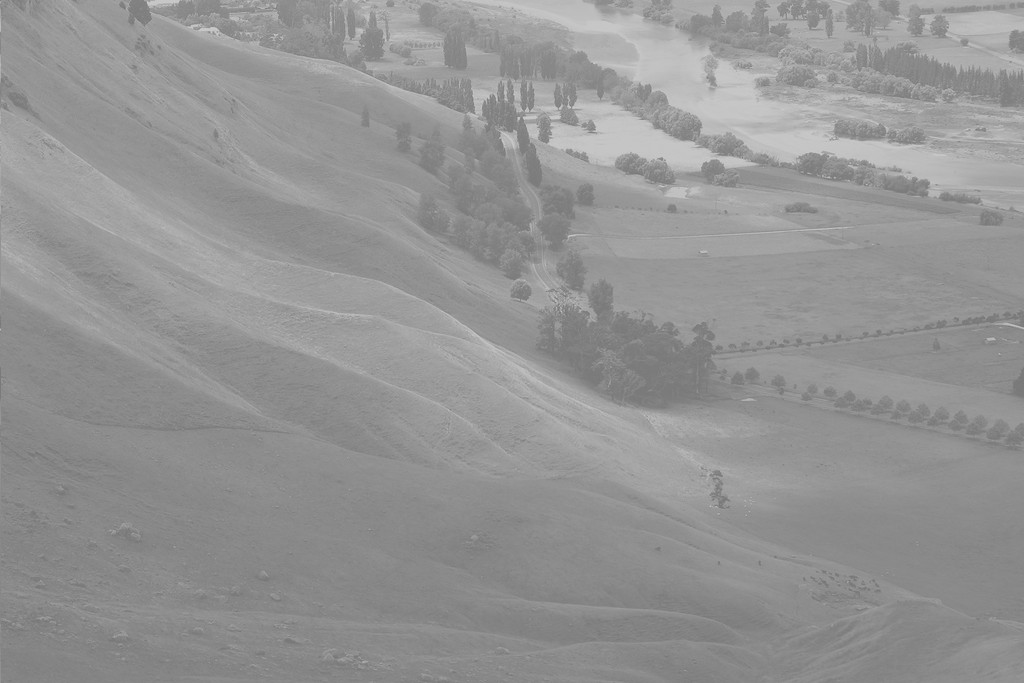
\includegraphics[width=\textwidth]{figuras/Unequalized.jpg}
      \subcaption*{(a)}
      \label{fig:unequalizedImage}
    \end{subfigure}
    \begin{subfigure}[t]{0.3\textwidth}
      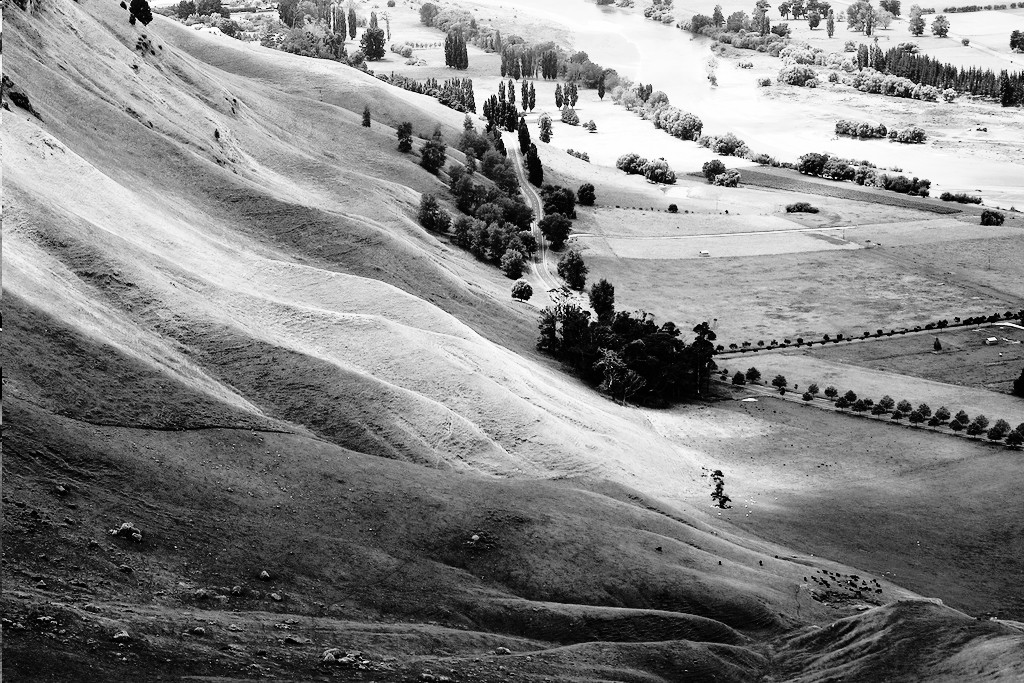
\includegraphics[width=\textwidth]{figuras/Equalized.jpg}
      \subcaption*{(b)}
      \label{fig:equalizedImage}
    \end{subfigure}
    \source{https://en.wikipedia.org/wiki/Histogram\_equalization}
    \caption{Exemplo do uso da equalização de histograma para realçar o terreno
            na imagem. (a) Imagem não equalizada. (b) Imagem equalizada.}
    \label{fig:equalization}
\end{figure}

\begin{figure}[H]
    \centering
    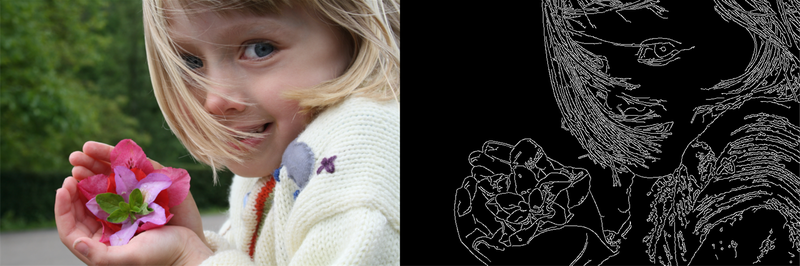
\includegraphics[width=0.8\textwidth]{figuras/canny.png}
    \source{https://en.wikipedia.org/wiki/Canny\_edge\_detector}
    \caption{Resultado do algoritmo de detecção de bordas Canny. A imagem à
    esquerda é a imagem de entrada, e a imagem à direita contém as bordas
    encontradas pelo Canny.}
    \label{fig:edgeDetection}
\end{figure}


%% ------------------------------------------------------------------------- %%
\subsection{Detecção de características}\index{Detecção de características}
\label{sec:dec_corr_carac}

  O próximo passo do registro é a detecção de características nas imagens de entrada.
As características, ou pontos de controle, são vetores de informações construídos
de tal maneira que cada característica representa unicamente a região na qual ela se
encontra. A construção do vetor de informação pode levar em conta só as intensidades
de um voxel por vez, procurar por regiões de alto contraste, como bordas, realizar
análises estatísticas em uma região ou formato ao redor de um ponto, entre outros
métodos.

  Em imagens médicas, normalmente uma característica pode ser representada por um ponto,
seja o centroide da região utilizada, ou a intersecção de retas. Logo, cada característica
é associada a uma posição $(x, y, z)$ da imagem. Exemplos de algoritmos para encontrar
características são \textit{Scale Invariant Feature Transform} (SIFT), introduzido por 
\cite{lowe2004distinctive}, e o \textit{Speeded Up Robust Features}
(SURF), desenvolvido por \cite{bay2008speeded}. Eles geram um vetor n-dimensional,
onde cada dimensão é construida a partir de uma propriedade invariante ao redor
de um ponto na imagem. As propriedades são invariantes à mudança de
orientação e iluminação. As características na figura \ref{fig:regExplicacao}(c) 
foram identificadas usando o SIFT.

%% ------------------------------------------------------------------------- %%
\subsection{Correspondência de características}\index{Correspondência de características}

  O próximo passo do registro é encontrar correspondências entre as características das
imagens. Este conjunto de pares é utilizado para encontrar um conjunto de parâmetros
pela função de transformação. As correspondência entre características na figura 
\ref{fig:regExplicacao}(d) foram identificadas usando o SIFT.

  O processo de correspondência pode ser melhorado levando-se em conta a possível
presença de ruido na etapa de detecção de características. Ele deve, ainda, encontrar
\textit{outliers}, ou seja, características que não tem correspondências, e eliminá-las 
do conjunto. Os seguintes algoritmos são exemplos da correspondência entre características 
de ponto:

\begin{description}
    \item [Clustering] Em casos onde as características são invariantes em relação
          a mudanças de orientação, metodologias de \textit{clustering} podem ser utilizadas
          para estabelecer relações entre os conjuntos de características;
    \item [Coerência espacial] Três pares de pontos não colineares nas duas imagens
          são escolhidos como base de uma transformação linear. Todos os outros
          pontos de um dos conjuntos passam pela mesma transformação e uma métrica
          é aplicada para calcular o quão bom foi o pareamento. Esse processo é repetido
          em busca da base que leva ao melhor pareamento;
\end{description}

%% ------------------------------------------------------------------------- %%
\subsection{Estimativa da função de deformação}\index{Estimativa da função de transformação}

  A função escolhida para deformar o espaço geométrico da imagem alvo deve ser
escolhida conforme a necessidade do problema a ser resolvido, a qualidade das
características encontradas, e a distribuição delas em torno das imagens. Com a
função de deformação escolhida, esse passo usa as correspondências encontradas
no passo anterior para definir os parâmetros utilizados pela função.

  Dada as coordenadas dos $N$ pares de correspondências entre pontos da imagem
referência e alvo, respectivamente:
\begin{equation}
  {(x_i, y_i, z_i), (X_i, Y_i, Z_i) : i = 1, \dots, N}
\end{equation}
  A função de deformação $f$ com componentes $f_x, f_y e f_z$ é definida como:
\begin{align}
  \begin{split}
    f_x(x, y, z) \approx X_i \\
    f_y(x, y, z) \approx Y_i \\
    f_z(x, y, z) \approx Z_i
  \end{split}
\end{align}

%% ------------------------------------------------------------------------- %%
\subsection{Re-amostragem da imagem Alvo}\index{Reamostragem da imagem Alvo}

  O último passo do registro é a re-amostragem da imagem alvo, ou a criação
da imagem registrada. Aplicando a função $f$ e seus parâmetros definidos pelo
passo anterior a todos os pontos da imagem alvo, temos o seguinte:

\begin{align}\label{eq:reamostragem}
    F(x_i, y_i, z_i) = A(I(f(x_i, y_i, z_i)))), \forall (i = 1, \dots, M)
\end{align}

  Onde $F(x_i, y_i, z_i)$ representa a posição $(x_i, y_i, z_i)$ nas imagens e
$M$ é a dimensão total das imagens.
  Como o resultado da função de deformação é continuo e as imagens estão em um
domínio discreto, uma função de interpolação, representada na equação \ref{eq:reamostragem}
por $I$, é aplicada. Algoritmos de interpolação como, por exemplo,
\textbf{Vizinhos próximos}, \textbf{Interpolação trilinear} ou \textbf{Splines Cúbicas}
são aplicados \cite{lehmann1999survey}.